\subsubsection{Interfaces}
zum einschalten der Interfaces habe ich im conf terminal des Routers einfachen die folgenden Befehle eingegeben:
\begin{lstlisting}
Router(config)#int range gig0/0-2
Router(config-if-range)#no shutdown
Router(config-if-range)#end
\end{lstlisting}
\begin{figure}[!htb]
    \centering
    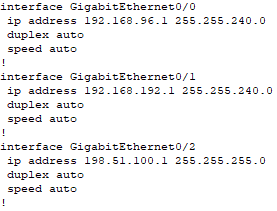
\includegraphics[width=\textwidth,height=.35\textwidth,keepaspectratio]{./img/config/interfaces.png}
    \caption{Running Config des Routers}
\end{figure}
\begin{figure}[!htb]
    \centering
    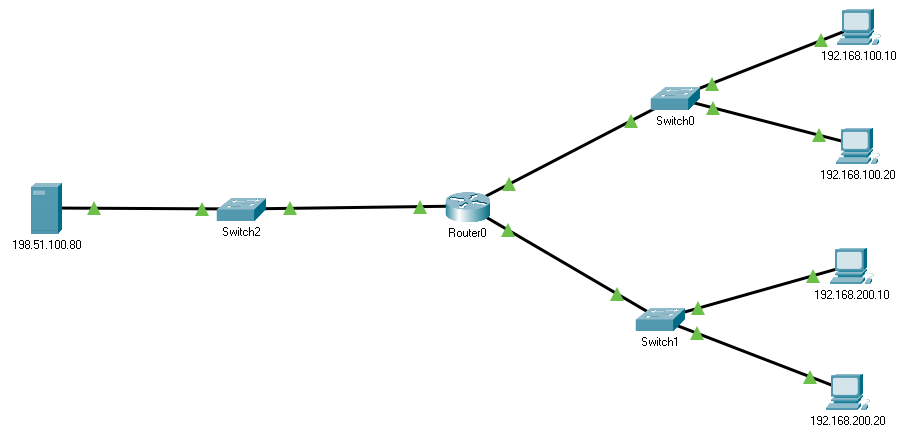
\includegraphics[width=\textwidth,height=.6\textwidth,keepaspectratio]{./img/config/end.png}
    \caption{Konfiguration nach einschalten des Routers}
\end{figure}
\FloatBarrier

\subsubsection{Frage 1}
\paragraph{Frage}
Wie kann die niedrigste freie Adresse in einem Netz errechnet werden,
und welche Adressen sind das in den gegebenen Netzen?
\paragraph{Antwort}
Man berechnet die Subnet Id zuerst. Dies wird ermöglicht in dem man die Netzmaske und die IP Adresse mit einem binären UND rechnet. Das Ergebnis wird um 1 erhöht und das ist die Adresse.\\
Die Berechnungen habe ich mit einem selbstgeschriebenem TS Programm durchgeführt.\\
Das Programm befindet sich zur Sicherheit im zip folder.\\
192.168.100.x/20 = 192.168.96.1 \\
192.168.200.x/20 = 192.168.192.1 \\
198.51.100.x/24 = 198.51.100.1
\begin{figure}[!htb]
    \centering
    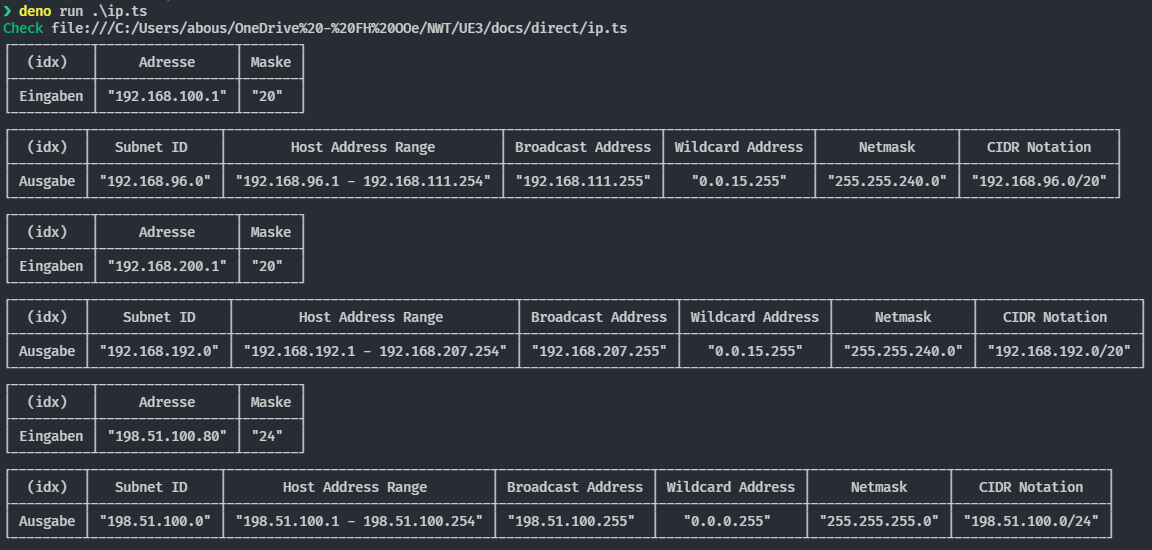
\includegraphics[width=\textwidth]{./img/config/frage1.png}
    \caption{Resultate der Berechnungen}
\end{figure}
\pagebreak

\subsubsection{IPv6}
Die Router Interfaces wurden über die CLI im conf terminal eingestellt.In dem Modus wählt man das jeweilige Interface und stellt mit ``ipv6 address xxx/64'' die Adresse ein.\\
Damit IPv6 Routing funktioniert muss im weiters im conf terminal des Routers IPv6 unicasting mit ``ipv6 unicast-routing'' aktiviert werden.\\
Der Server wurde über die GUI engestellt.
\begin{figure}[!htb]
    \centering
    \begin{subfigure}{.49\textwidth}
        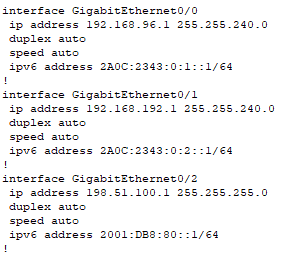
\includegraphics[width=\textwidth,height=.7\textwidth,keepaspectratio]{./img/config/router_ipv6.png}
        \caption{Router nach IPv6}
    \end{subfigure}
    \begin{subfigure}{.49\textwidth}
        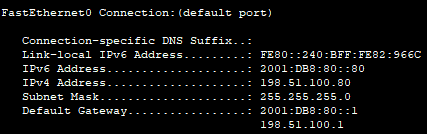
\includegraphics[width=\textwidth,height=.4\textwidth,keepaspectratio]{./img/config/server.png}
        \caption{Server}
    \end{subfigure}
\end{figure}


\subsubsection{Endsysteme}
Die PCs wurden über die GUI eingestellt.
\begin{figure}[!htb]
    \centering
    \begin{subfigure}{.49\textwidth}
        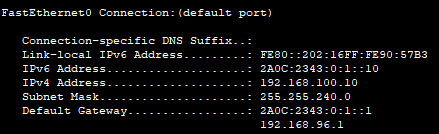
\includegraphics[width=\textwidth,height=.85\textwidth,keepaspectratio]{./img/config/pc0.png}
        \caption{Group 1 - PC1}
    \end{subfigure}
    \begin{subfigure}{.49\textwidth}
        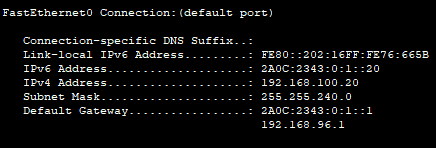
\includegraphics[width=\textwidth,height=.85\textwidth,keepaspectratio]{./img/config/pc1.png}
        \caption{Group 1 - PC2}
    \end{subfigure}
    ~
    \begin{subfigure}{.49\textwidth}
        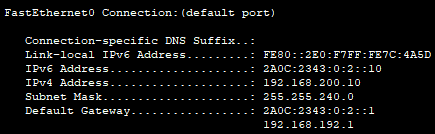
\includegraphics[width=\textwidth,height=.88\textwidth,keepaspectratio]{./img/config/pc2.png}
        \caption{Group 2 - PC1}
    \end{subfigure}
    \begin{subfigure}{.49\textwidth}
        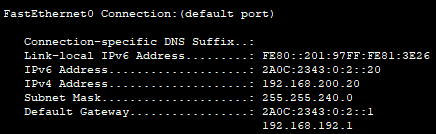
\includegraphics[width=\textwidth,height=.88\textwidth,keepaspectratio]{./img/config/pc3.png}
        \caption{Group 2 - PC2}
    \end{subfigure}
    \caption{IP-Config}
\end{figure}
\FloatBarrier
\paragraph{Tests}
\begin{figure}[!htb]
    \centering
    \begin{subfigure}{.49\textwidth}
        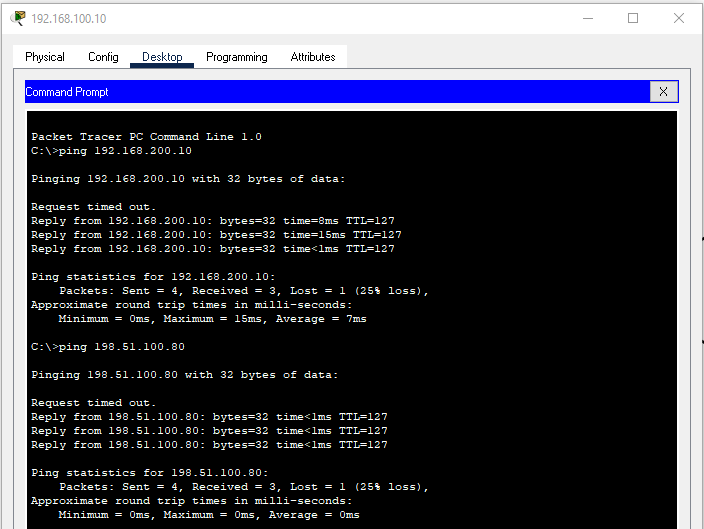
\includegraphics[width=\textwidth,height=.85\textwidth,keepaspectratio]{./img/config/test1.png}
        \caption{Group 1 zu Group 2 und Server}
    \end{subfigure}
    \begin{subfigure}{.49\textwidth}
        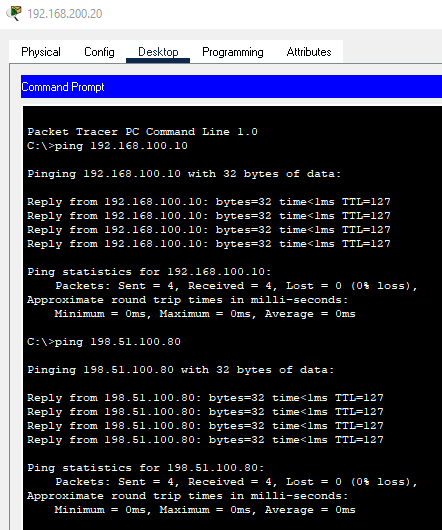
\includegraphics[width=\textwidth,height=.85\textwidth,keepaspectratio]{./img/config/test2.png}
        \caption{Group 2 zu Group 1 und Server}
    \end{subfigure}
    \caption{IPv4 Kommunikation}
\end{figure}

\begin{figure}[!htb]
    \centering
    \begin{subfigure}{.49\textwidth}
        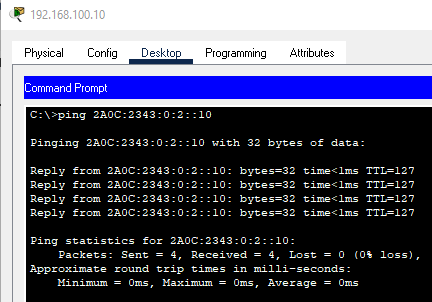
\includegraphics[width=\textwidth,height=.88\textwidth,keepaspectratio]{./img/config/test_ipv6.png}
        \caption{Group 1 zu Group 2 ping}
    \end{subfigure}
    \begin{subfigure}{.49\textwidth}
        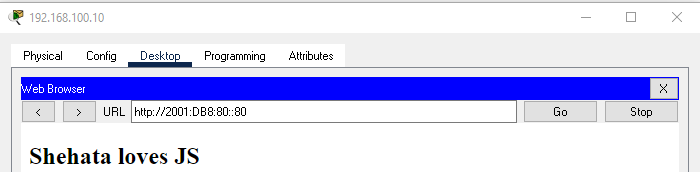
\includegraphics[width=\textwidth,height=.88\textwidth,keepaspectratio]{./img/config/test_server.png}
        \caption{Kommunikation zum Server über den Browser}
    \end{subfigure}
    \caption{IPv6 Kommunikation}
\end{figure}
\pagebreak

\subsubsection{Frage 2}
\paragraph{Frage}
Warum funktioniert das, obwohl noch keine Routen gesetzt wurden?
\paragraph{Antwort}
Weil der Router direkt mit den Systemen verbunden ist, erkennt er die Subnet Id automatisch und kann die Adressen routen.
\begin{figure}[!htb]
    \centering
    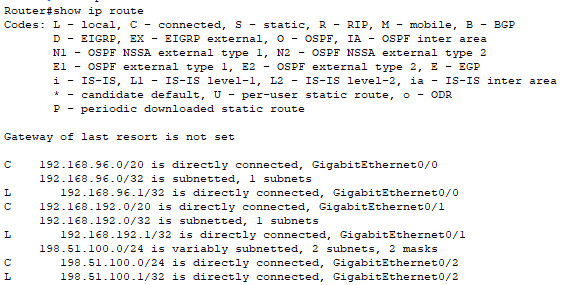
\includegraphics[width=\textwidth,height=.4\textwidth,keepaspectratio]{./img/config/ip_route.png}
    \caption{IPv4 Routes des Routers}
    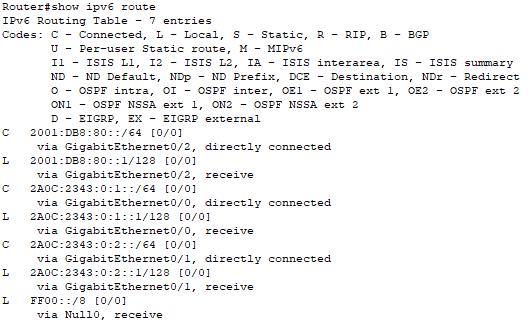
\includegraphics[width=\textwidth,height=.5\textwidth,keepaspectratio]{./img/config/ipv6_route.png}
    \caption{IPv6 Routes des Routers}
\end{figure}